\documentclass[./../../paper.tex]{subfiles}
\graphicspath{{\subfix{./../../figures/}}}

\begin{document}


\label{sec:exp1}
As there are many ways to combine each configuration, we select a few configurations by examining them trough simulations.  



The model-configuration set contains \attention{144} elements. We choose to run each model-configuration for \attention{50} evolution cycles. For all model-configurations, we use the same set of \attention{4} factual \glspl{instance}, which are randomly sampled from the test set. We ensure, that the outcomes of these factuals are evenly divided. We decide to return a maximum of \attention{1000} counterfactuals for each factual case. Within each evolutionary cycle, we generate \attention{100} new offsprings. We keep the mutation rate at \attention{0.1} for each mutation type. Hence, across all cases that are mutated, the algorithm deletes, inserts, and changes \attention{1\%} of events. We collect the means viability and its components across the iterative cycles of the model.

% After retrieving the results, we fit a linear mixed-effects model to determine the importance of each model-configuration. Here, we use the resulting viability as a dependent variable and each phase as independent variable. We adjust the model according to their model-configuration, as we retrieve \attention{50} samples per model-configuration. If a phase-type strongly affects the dependent variable and the resulting change is deemed significant, we can draw conclusions about the full model-configuration. Furthermore, preliminary results showed that many of the model-configurations have a zero feasibility. Hence, we also incorporate the insights gained from using feasibility as a dependent variable.

% \subsection{Results}

% TODO: Change plots to matplotlib plots
\begin{figure}[htbp]
    \centering
    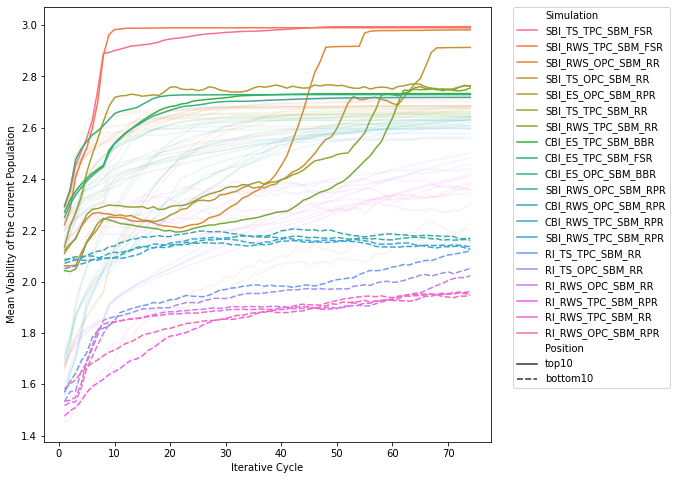
\includegraphics[width=\textwidth]{figures/generated/exp1_effect_on_viability_top10_last10.png}
    \caption{This figure shows the average viability of the \attention{10} best and worst model-configurations. The x-axis shows how the viability evolves for each evolutionary cycle.}
    \label{fig:average-viability}
\end{figure}

\noindent \autoref{fig:average-viability} shows the bottom and top-\attention{k} model-configurations based on the viability after the final iterative cycle. We also show how the viability evolves for each iteration.\attention{change evolutionary cycle to iterative cycle} The results reveal a couple of patterns. 
First, all of the top-\attention{k} algorithms use \attention{either CaseBasedInitiator or SampleBasedInitiator} as initiation operation. In contrast, the bottom-\attention{k} all use \attention{RandomInitiator} as initialisation. 
Second, we see that most of the top-\attention{k} algorithms use the \attention{ElitismSelector}. 

The complete table of results are in \autoref{tbl:average-viability}.
% \needsattachment{tbl:average-viability}

% \noindent  shows for the \attention{average feasibility for each model-configuration}. It does not surprise, that the \attention{FactualInitiator} remains at a low feasibility as deviations will often lead to infeasible counterfactuals. The evolutionary algorithm remains at a local optimum without exploring other solutions. Furthermore, we see that most model-configurations reach at most \attention{0.04} feasibility, while the initialisation with the \attention{DataDistributionSample} initiator reaches higher values. 


% \graphicspath{{\subfix{./../../figures/}}}

\begin{figure}[htbp]
    \centering
    \begin{subfigure}[c]{0.9\textwidth}
        \centering
        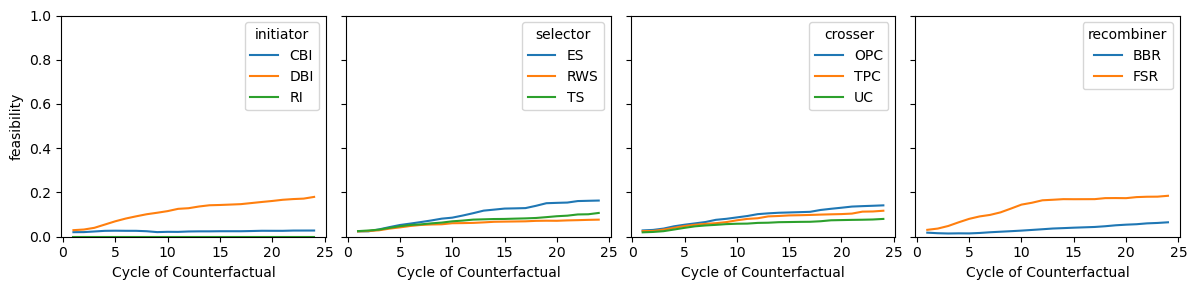
\includegraphics[width=\textwidth]{figures/generated/exp1_feasibility.png}
        \label{fig:exp1-feasibility}    
    \end{subfigure}
    \hfill
    \begin{subfigure}[c]{0.9\textwidth}
        \centering
        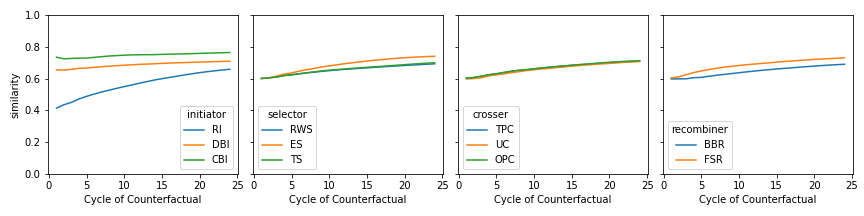
\includegraphics[width=\textwidth]{figures/generated/exp1_similarity.png}
        \label{fig:exp1-similarity}
    \end{subfigure}
    \hfill
    \begin{subfigure}[c]{0.9\textwidth}
        \centering
        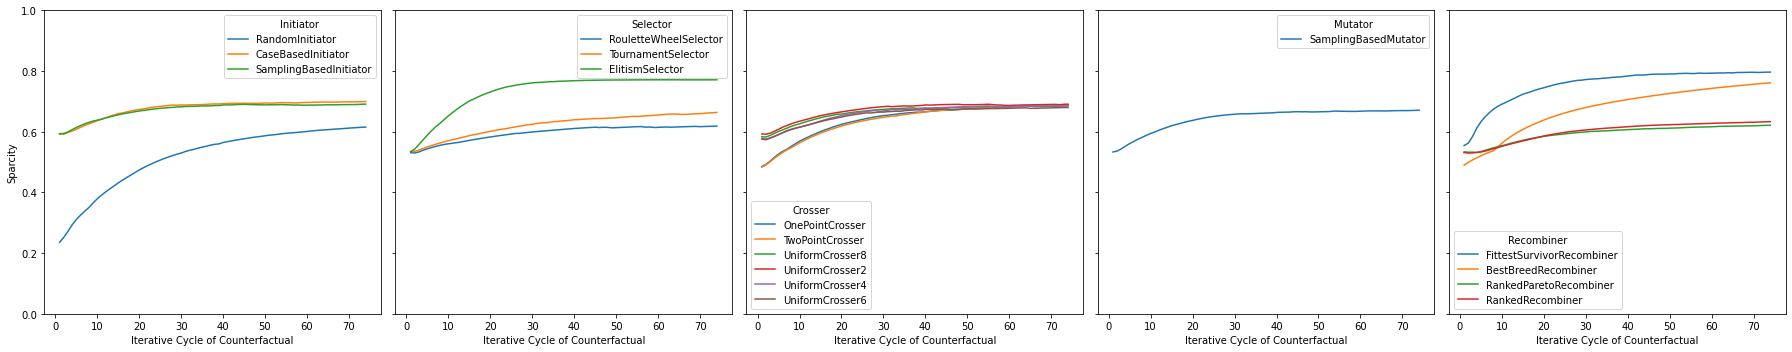
\includegraphics[width=\textwidth]{figures/generated/exp1_sparcity.png}
        \label{fig:exp1-sparcity}
    \end{subfigure}
    \hfill
    \begin{subfigure}[c]{0.9\textwidth}
        \centering
        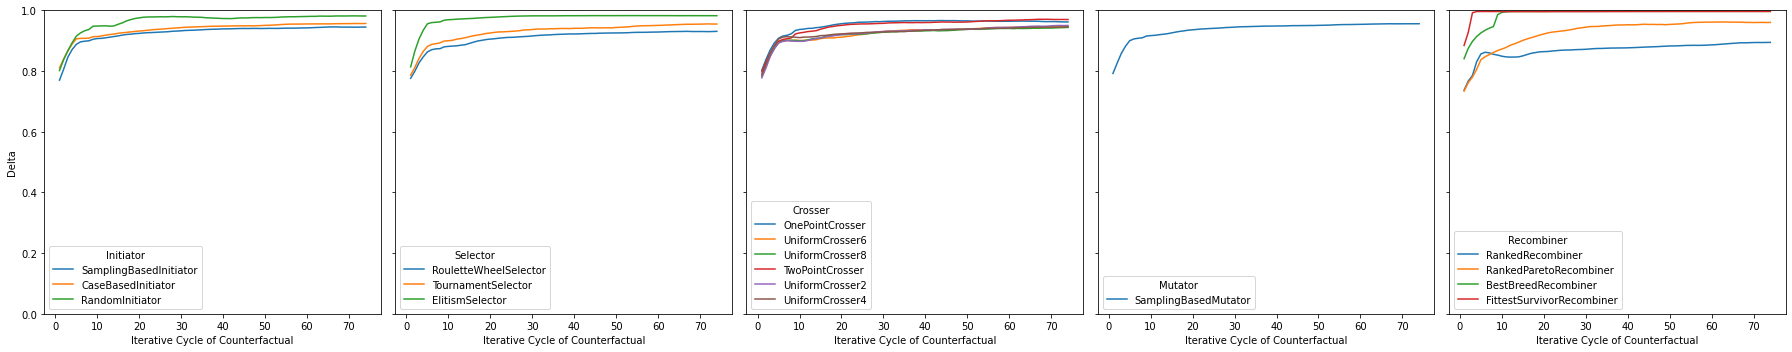
\includegraphics[width=\textwidth]{figures/generated/exp1_delta.png}
        \label{fig:exp1-delta}
    \end{subfigure}
    \caption{The evolution of each viability measure over the entire span of iterative cycles. Each figure adjust the respective operator type by taking the average over all other operator types. \attention{Make sure, that the legends are aligned in color.}}
    \label{fig:exp1-measure}
\end{figure}

\xixi{Shall I discuss the big figure or just viability in this section?} In \autoref{fig:exp1-measure}, we see the effects of each operator type, except the mutation operation. 

Starting with some commonalities across operator-type and measure, the figure shows that the initiator heavily determines the starting point for each measure. For instance, the \attention{RandomInitiator} starts well below the other initiator operations when it comes to sparcity and similarity. 
Another noteworthy general observation is the delta measure\attention{Change some of the names to align with Dice4EL}. Here, for each operator type we see a movement towards the highest possible delta value. Hence, most configurations are capable of changing the source class to the desired class. 

In terms of viability \autoref{fig:exp1-feasibility}, shows an increase only for cases, in which the \attention{SampleBasedInitiator} is used. Similar holds for recombination with \attention{FittestSurvivorRecombiner}.

The results for the selection operator type are undeniably in favor of \attention{ElitismSelector} for all viability measures. The same holds for the recombination operation. Here, the \attention{FittestSurvivorRecombiner} yields better results.

When it comes to the crossing operation, the results indicate, the differences between \attention{OnePointCrosser} and \attention{TwoPointCrosser} are inconclusive for all viability measures except feasibility. One can explain that by noting, that both operations are very similar in nature. However, cutting the sequence only once retains produces less impossible sequences for the child sequences.






\end{document}